\section{Hybrid System}
\label{sec:hybrid_system}

\subsection{Q3.1: Filament Replacement}
\label{sec:q31}

\todo[inline]{Hybrid model: state, inputs, modes, events, invariants, guards and reset maps (tables).}

\begin{figure}[H]
    \centering
    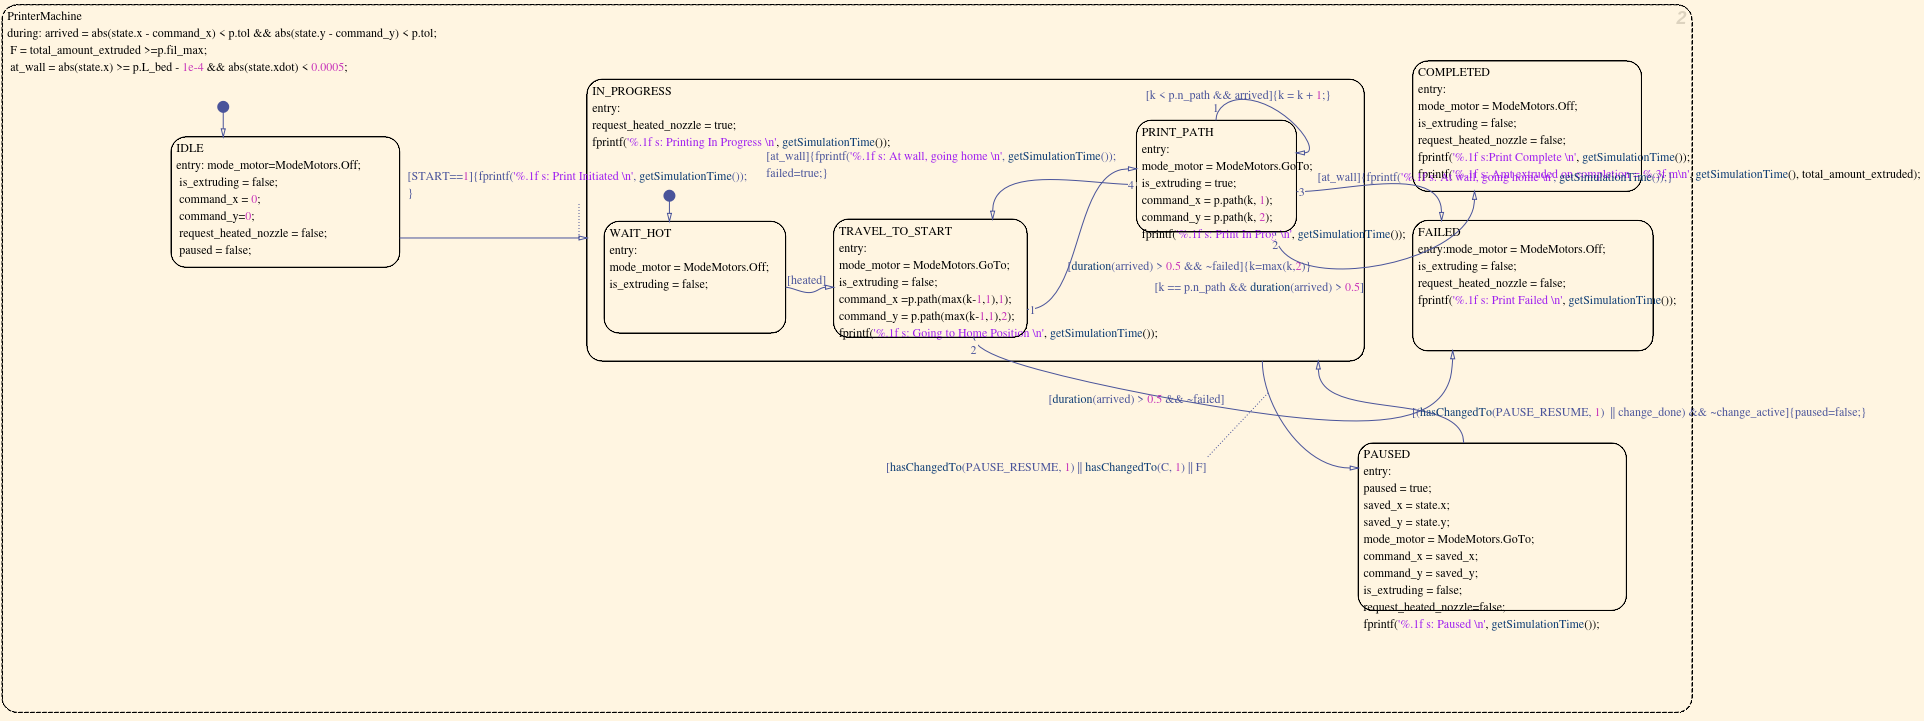
\includegraphics[width=\textwidth]{figures/q31/stateflow_printer.png}
    \caption{Stateflow chart of the printer machine.}
    \label{fig:q31_chart_printer}
\end{figure}

\begin{figure}[H]
    \centering
    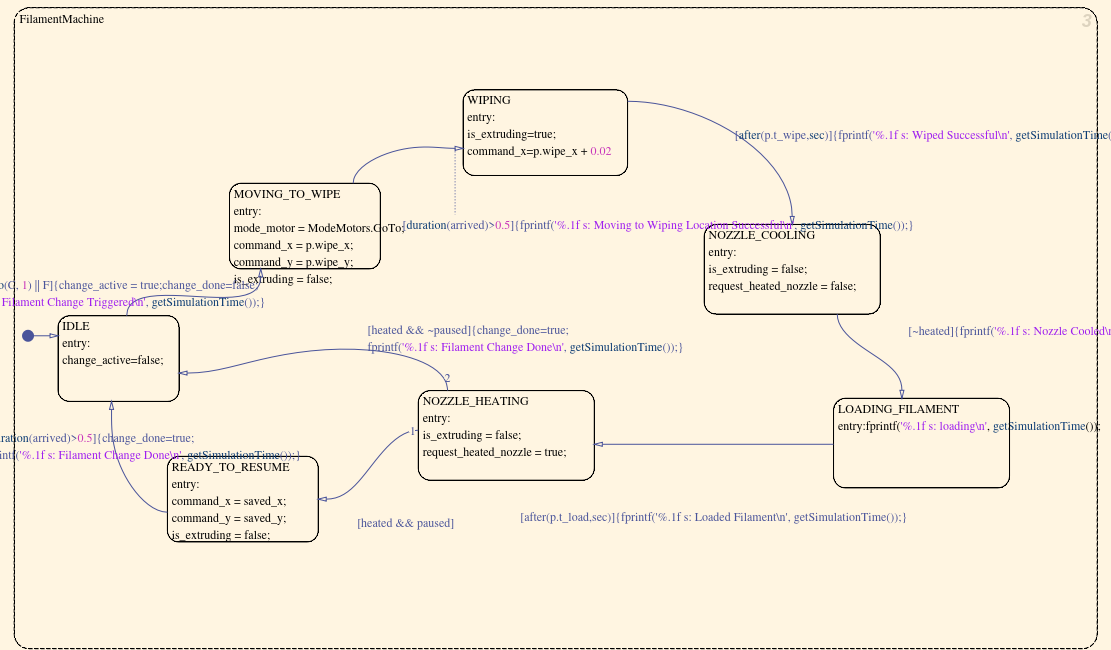
\includegraphics[width=0.8\textwidth]{figures/q31/stateflow_filament.png}
    \caption{Stateflow chart of the filament machine.}
    \label{fig:q31_chart_filament}
\end{figure}

\todo[inline]{Simulation setup: square path, $L_{spool}$, the instants at which $C$ and $F$ are applied.}

\subsubsection{Case 1: Colour Change}
\label{sec:q31_case1}
\todo[inline]{Scenario: $C$ is applied at $t\approx\SI{69.6}{s}$ while printing; the head moves to the wipe location, wipes, loads the new filament, reheats and resumes (red to green). The run completes at $t\approx\SI{163}{s}$.}

\begin{figure}[H]
    \centering
    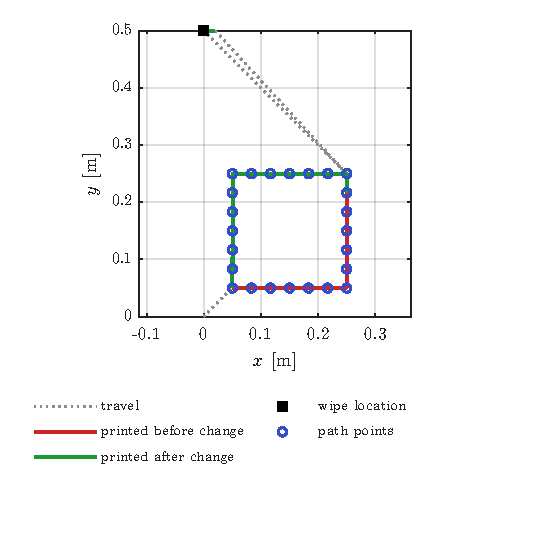
\includegraphics[width=0.55\textwidth]{figures/q31/case1_colour_change/1_head_path.pdf}
    \caption{Case 1. Head path: printed before the change (red), after (green), and travel moves.}
    \label{fig:q31_case1_path}
\end{figure}

\begin{figure}[H]
    \centering
    \begin{subfigure}[t]{\textwidth}
        \centering
        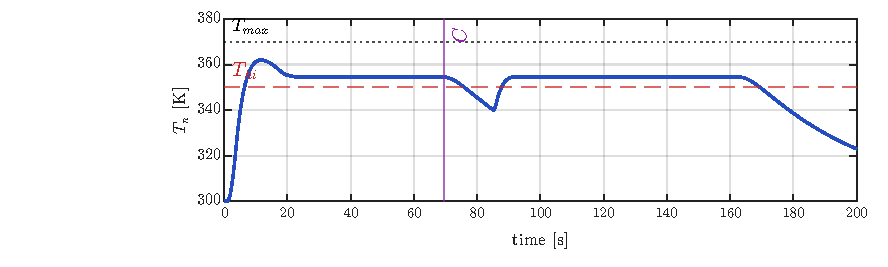
\includegraphics[width=0.95\linewidth]{figures/q31/case1_colour_change/2_nozzle_temperature.pdf}
        \caption{Nozzle temperature $T_n$ with the thresholds $T_{hi}$ and $T_{max}$.}
    \end{subfigure}
    \begin{subfigure}[t]{\textwidth}
        \centering
        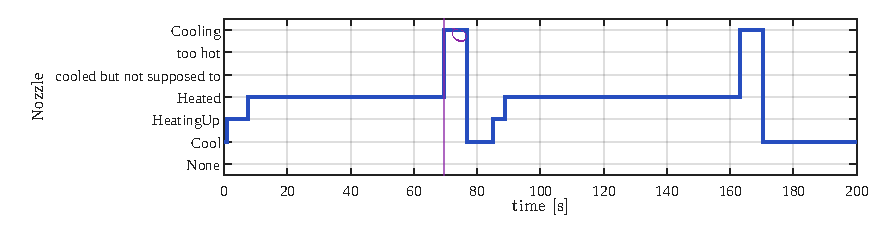
\includegraphics[width=0.95\linewidth]{figures/q31/case1_colour_change/3_nozzle_mode.pdf}
        \caption{Nozzle machine.}
    \end{subfigure}
    \begin{subfigure}[t]{\textwidth}
        \centering
        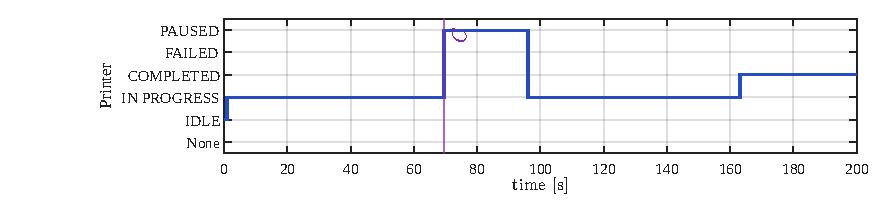
\includegraphics[width=0.95\linewidth]{figures/q31/case1_colour_change/4_printer_mode.pdf}
        \caption{Printer machine.}
    \end{subfigure}
    \begin{subfigure}[t]{\textwidth}
        \centering
        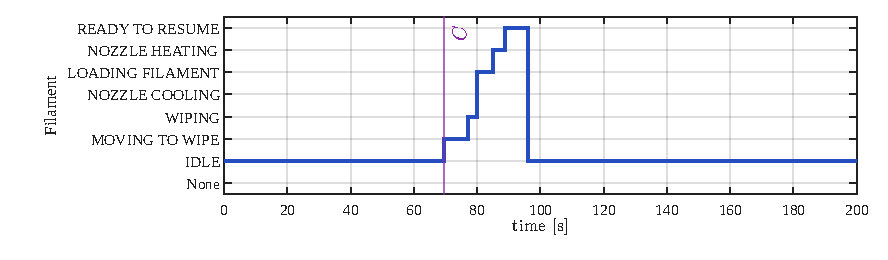
\includegraphics[width=0.95\linewidth]{figures/q31/case1_colour_change/5_filament_mode.pdf}
        \caption{Filament machine.}
    \end{subfigure}
    \begin{subfigure}[t]{\textwidth}
        \centering
        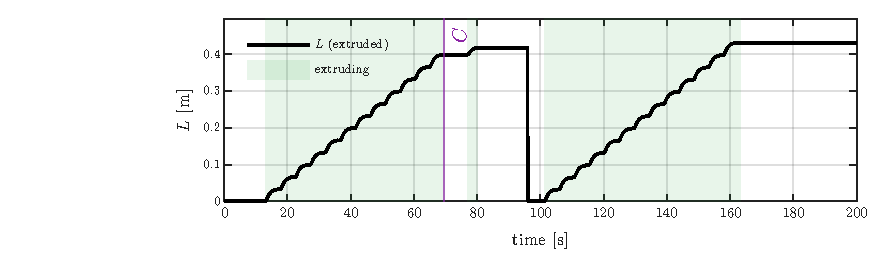
\includegraphics[width=0.95\linewidth]{figures/q31/case1_colour_change/6_filament_extruded.pdf}
        \caption{Extruded filament length $L$ against $L_{spool}$.}
    \end{subfigure}
    \caption{Case 1. Nozzle temperature, machine modes and extruded length.}
    \label{fig:q31_case1_modes}
\end{figure}

\subsubsection{Case 2: Filament Runout}
\label{sec:q31_case2}
\todo[inline]{Scenario: the spool runs out ($F$) at $t\approx\SI{69.6}{s}$, and again at $t\approx\SI{158}{s}$ after the first replacement, so the filament sequence runs twice. The run completes at $t\approx\SI{191}{s}$.}

\begin{figure}[H]
    \centering
    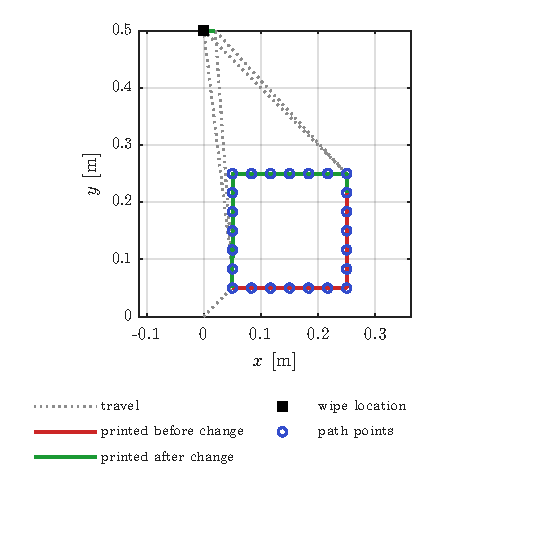
\includegraphics[width=0.55\textwidth]{figures/q31/case2_filament_runout/1_head_path.pdf}
    \caption{Case 2. Head path: printed before the change (red), after (green), and travel moves.}
    \label{fig:q31_case2_path}
\end{figure}

\begin{figure}[H]
    \centering
    \begin{subfigure}[t]{\textwidth}
        \centering
        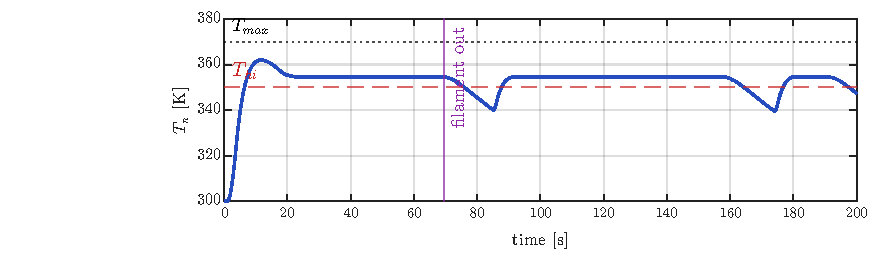
\includegraphics[width=0.95\linewidth]{figures/q31/case2_filament_runout/2_nozzle_temperature.pdf}
        \caption{Nozzle temperature $T_n$ with the thresholds $T_{hi}$ and $T_{max}$.}
    \end{subfigure}
    \begin{subfigure}[t]{\textwidth}
        \centering
        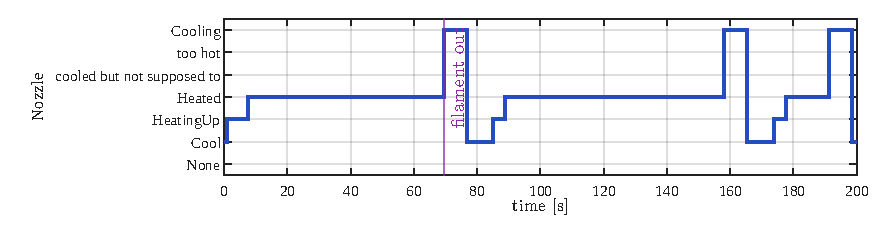
\includegraphics[width=0.95\linewidth]{figures/q31/case2_filament_runout/3_nozzle_mode.pdf}
        \caption{Nozzle machine.}
    \end{subfigure}
    \begin{subfigure}[t]{\textwidth}
        \centering
        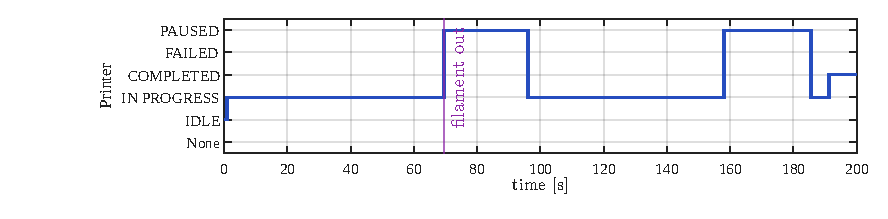
\includegraphics[width=0.95\linewidth]{figures/q31/case2_filament_runout/4_printer_mode.pdf}
        \caption{Printer machine.}
    \end{subfigure}
    \begin{subfigure}[t]{\textwidth}
        \centering
        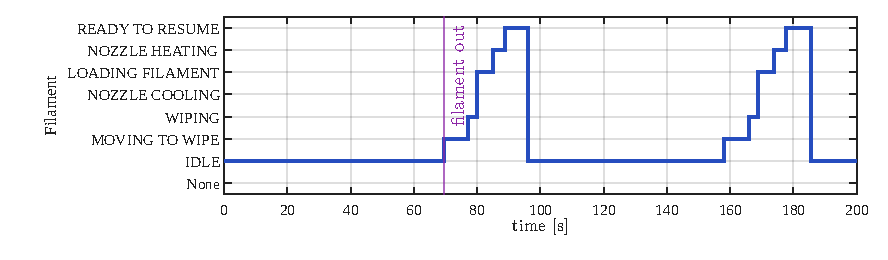
\includegraphics[width=0.95\linewidth]{figures/q31/case2_filament_runout/5_filament_mode.pdf}
        \caption{Filament machine.}
    \end{subfigure}
    \begin{subfigure}[t]{\textwidth}
        \centering
        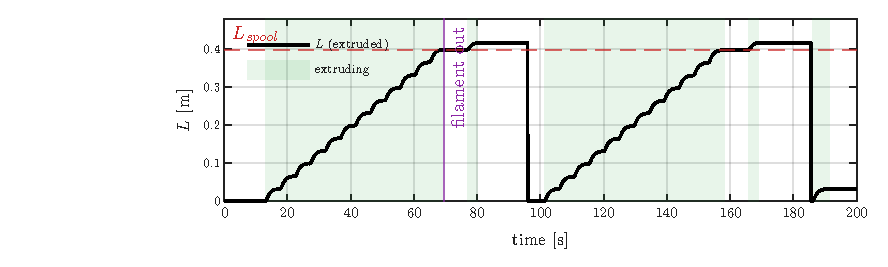
\includegraphics[width=0.95\linewidth]{figures/q31/case2_filament_runout/6_filament_extruded.pdf}
        \caption{Extruded filament length $L$ against $L_{spool}$.}
    \end{subfigure}
    \caption{Case 2. Nozzle temperature, machine modes and extruded length.}
    \label{fig:q31_case2_modes}
\end{figure}

\subsubsection{Discussion}
\todo[inline]{Compare both cases with the FSM of Chapter~2: order of filament states, nozzle cooling and reheating, resumption point.}

\subsection{Q3.2: Drawing a Square}
\label{sec:q32}

\todo[inline]{Draw the square using only the motor angle sensors; add the rotated square (bonus).}
